
%	-------------------------------------------------------------------------------
% 
%
%
%
%
%
%
%
%
%
%	-------------------------------------------------------------------------------

	\documentclass[12pt, a4paper, oneside]{book}
%	\documentclass[12pt, a4paper, landscape, oneside]{book}

		% --------------------------------- 페이지 스타일 지정
		\usepackage{geometry}
%		\geometry{landscape=true	}
		\geometry{top 		=10em}
		\geometry{bottom		=10em}
		\geometry{left		=8em}
		\geometry{right		=8em}
		\geometry{headheight	=4em} % 머리말 설치 높이
		\geometry{headsep		=2em} % 머리말의 본문과의 띠우기 크기
		\geometry{footskip		=4em} % 꼬리말의 본문과의 띠우기 크기
% 		\geometry{showframe}
	
%		paperwidth 	= left + width + right (1)
%		paperheight 	= top + height + bottom (2)
%		width 		= textwidth (+ marginparsep + marginparwidth) (3)
%		height 		= textheight (+ headheight + headsep + footskip) (4)



		%	===================================================================
		%	package
		%	===================================================================
%			\usepackage[hangul]{kotex}				% 한글 사용
			\usepackage{kotex}					% 한글 사용
			\usepackage[unicode]{hyperref}			% 한글 하이퍼링크 사용

		% ------------------------------ 수학 수식
			\usepackage{amssymb,amsfonts,amsmath}	% 수학 수식 사용
			\usepackage{mathtools}				% amsmath 확장판

			\usepackage{scrextend}				% 
		

		% ------------------------------ LIST
			\usepackage{enumerate}			%
			\usepackage{enumitem}			%
			\usepackage{tablists}				%	수학문제의 보기 등을 표현하는데 사용
										%	tabenum


		% ------------------------------ table 
			\usepackage{longtable}			%
			\usepackage{tabularx}			%
			\usepackage{tabu}				%




		% ------------------------------ 
			\usepackage{setspace}			%
			\usepackage{booktabs}		% table
			\usepackage{color}			%
			\usepackage{multirow}			%
			\usepackage{boxedminipage}	% 미니 페이지
			\usepackage[pdftex]{graphicx}	% 그림 사용
			\usepackage[final]{pdfpages}		% pdf 사용
			\usepackage{framed}			% pdf 사용

			
			\usepackage{fix-cm}	
			\usepackage[english]{babel}

		% ------------------------------ 음악
%			\usepackage{kslilymusic}			%
%			\usepackage{lyluatex}
	
		%	=======================================================================================
		% 	tikz package
		% 	
		% 	--------------------------------- 	
			\usepackage{tikz}%
			\usetikzlibrary{arrows,positioning,shapes}
			\usetikzlibrary{mindmap}			
			

		% --------------------------------- 	page
			\usepackage{afterpage}		% 다음페이지가 나온면 어떻게 하라는 명령 정의 패키지
%			\usepackage{fullpage}			% 잘못 사용하면 다 흐트러짐 주의해서 사용
%			\usepackage{pdflscape}		% 
			\usepackage{lscape}			%	 


			\usepackage{blindtext}
	
		% --------------------------------- font 사용
			\usepackage{pifont}				%
			\usepackage{textcomp}
			\usepackage{gensymb}
			\usepackage{marvosym}



		% Package --------------------------------- 

			\usepackage{tablists}				%


		% Package --------------------------------- 
			\usepackage[framemethod=TikZ]{mdframed}				% md framed package
			\usepackage{smartdiagram}								% smart diagram package



		% Package ---------------------------------    연습문제 

			\usepackage{exsheets}				%

			\SetupExSheets{solution/print=true}
			\SetupExSheets{question/type=exam}
			\SetupExSheets[points]{name=point,name-plural=points}


		% --------------------------------- 페이지 스타일 지정

		\usepackage[Sonny]		{fncychap}

			\makeatletter
			\ChNameVar	{\Large\bf}
			\ChNumVar	{\Huge\bf}
			\ChTitleVar		{\Large\bf}
			\ChRuleWidth	{0.5pt}
			\makeatother

%		\usepackage[Lenny]		{fncychap}
%		\usepackage[Glenn]		{fncychap}
%		\usepackage[Conny]		{fncychap}
%		\usepackage[Rejne]		{fncychap}
%		\usepackage[Bjarne]	{fncychap}
%		\usepackage[Bjornstrup]{fncychap}

		\usepackage{fancyhdr}
		\pagestyle{fancy}
		\fancyhead{} % clear all fields
		\fancyhead[LO]{\footnotesize \leftmark}
		\fancyhead[RE]{\footnotesize \leftmark}
		\fancyfoot{} % clear all fields
		\fancyfoot[LE,RO]{\large \thepage}
		%\fancyfoot[CO,CE]{\empty}
		\renewcommand{\headrulewidth}{1.0pt}
		\renewcommand{\footrulewidth}{0.4pt}
	
	
	
		%	--------------------------------------------------------------------------------------- 
		% 	tritlesec package
		% 	
		% 	
		% 	------------------------------------------------------------------ section 스타일 지정
	
			\usepackage{titlesec}
		
		% 	----------------------------------------------------------------- section 글자 모양 설정
			\titleformat*{\section}					{\large\bfseries}
			\titleformat*{\subsection}				{\normalsize\bfseries}
			\titleformat*{\subsubsection}			{\normalsize\bfseries}
			\titleformat*{\paragraph}				{\normalsize\bfseries}
			\titleformat*{\subparagraph}				{\normalsize\bfseries}
	
		% 	----------------------------------------------------------------- section 번호 설정
			\renewcommand{\thepart}				{\arabic{part}.}
			\renewcommand{\thesection}				{\arabic{section}.}
			\renewcommand{\thesubsection}			{\thesection\arabic{subsection}.}
			\renewcommand{\thesubsubsection}		{\thesubsection\arabic{subsubsection}}
			\renewcommand\theparagraph 			{$\blacksquare$ \hspace{3pt}}

		% 	----------------------------------------------------------------- section 페이지 나누기 설정
			\let\stdsection\section
			\renewcommand\section{\newpage\stdsection}



		%	--------------------------------------------------------------------------------------- 
		% 	\titlespacing*{commandi} {left} {before-sep} {after-sep} [right-sep]		
		% 	left
		%	before-sep		:  수직 전 간격
		% 	after-sep	 	:  수직으로 후 간격
		%	right-sep

			\titlespacing*{\section} 			{0pt}{1.0em}{1.0em}
			\titlespacing*{\subsection}	  		{0ex}{1.0em}{1.0em}
			\titlespacing*{\subsubsection}		{0ex}{1.0em}{1.0em}
			\titlespacing*{\paragraph}			{0em}{1.5em}{1.0em}
			\titlespacing*{\subparagraph}		{4em}{1.0em}{1.0em}
	
		%	\titlespacing*{\section} 			{0pt}{0.0\baselineskip}{0.0\baselineskip}
		%	\titlespacing*{\subsection}	  		{0ex}{0.0\baselineskip}{0.0\baselineskip}
		%	\titlespacing*{\subsubsection}		{6ex}{0.0\baselineskip}{0.0\baselineskip}
		%	\titlespacing*{\paragraph}			{6pt}{0.0\baselineskip}{0.0\baselineskip}
	

		% --------------------------------- recommend		섹션별 페이지 상단 여백
		\newcommand{\SectionMargin}				{\newpage  \null \vskip 2cm}
		\newcommand{\SubSectionMargin}			{\newpage  \null \vskip 2cm}
		\newcommand{\SubSubSectionMargin}		{\newpage  \null \vskip 2cm}


		%	--------------------------------------------------------------------------------------- 
		% 	toc 설정  - table of contents
		% 	
		% 	
		% 	----------------------------------------------------------------  문서 기본 사항 설정
			\setcounter{secnumdepth}{4} 		% 문단 번호 깊이
			\setcounter{tocdepth}{2} 			% 문단 번호 깊이 - 목차 출력시 출력 범위

			\setlength{\parindent}{0cm} 		% 문서 들여 쓰기를 하지 않는다.


		%	--------------------------------------------------------------------------------------- 
		% 	mini toc 설정
		% 	
		% 	
		% 	--------------------------------------------------------- 장의 목차  minitoc package
			\usepackage{minitoc}

			\setcounter{minitocdepth}{1}    	%  Show until subsubsections in minitoc
%			\setlength{\mtcindent}{12pt} 	% default 24pt
			\setlength{\mtcindent}{24pt} 	% default 24pt

		% 	--------------------------------------------------------- part toc
		%	\setcounter{parttocdepth}{2} 	%  default
			\setcounter{parttocdepth}{0}
		%	\setlength{\ptcindent}{0em}		%  default  목차 내용 들여 쓰기
			\setlength{\ptcindent}{0em}         


		% 	--------------------------------------------------------- section toc

			\renewcommand{\ptcfont}{\normalsize\rm} 		%  default
			\renewcommand{\ptcCfont}{\normalsize\bf} 	%  default
			\renewcommand{\ptcSfont}{\normalsize\rm} 	%  default


		%	=======================================================================================
		% 	tocloft package
		% 	
		% 	------------------------------------------ 목차의 목차 번호와 목차 사이의 간격 조정
			\usepackage{tocloft}

		% 	------------------------------------------ 목차의 내어쓰기 즉 왼쪽 마진 설정
			\setlength{\cftsecindent}{2em}			%  section

		% 	------------------------------------------ 목차의 목차 번호와 목차 사이의 간격 조정
			\setlength{\cftsecnumwidth}{2em}		%  section





		%	=======================================================================================
		% 	flowchart  package
		% 	
		% 	------------------------------------------ 목차의 목차 번호와 목차 사이의 간격 조정
			\usepackage{flowchart}
			\usetikzlibrary{arrows}



		%	=======================================================================================
		% 	줄 간격 설정
		% 	
		% 	
		% 	--------------------------------- 	줄간격 설정
			\doublespace
%			\onehalfspace
%			\singlespace
		
		

	% 	============================================================================== itemi Global setting

	
		%	-------------------------------------------------------------------------------
		%		Vertical spacing
		%	-------------------------------------------------------------------------------
			\setlist[itemize]{topsep=0.0em}			% 상단의 여유치
			\setlist[itemize]{partopsep=0.0em}			% 
			\setlist[itemize]{parsep=0.0em}			% 
%			\setlist[itemize]{itemsep=0.0em}			% 
			\setlist[itemize]{noitemsep}				% 
			
		%	-------------------------------------------------------------------------------
		%		Horizontal spacing
		%	-------------------------------------------------------------------------------
			\setlist[itemize]{labelwidth=1em}			%  라벨의 표시 폭
			\setlist[itemize]{leftmargin=8em}			%  본문 까지의 왼쪽 여백  - 4em
			\setlist[itemize]{labelsep=3em} 			%  본문에서 라벨까지의 거리 -  3em
			\setlist[itemize]{rightmargin=0em}			% 오른쪽 여백  - 4em
			\setlist[itemize]{itemindent=0em} 			% 점 내민 거리 label sep 과 같은면 점위치 까지 내민다
			\setlist[itemize]{listparindent=3em}		% 본문 드려쓰기 간격
	
	
			\setlist[itemize]{ topsep=0.0em, 			%  상단의 여유치
						partopsep=0.0em, 		%  
						parsep=0.0em, 
						itemsep=0.0em, 
						labelwidth=1em, 
						leftmargin=2.5em,
						labelsep=2em,			%  본문에서 라벨 까지의 거리
						rightmargin=0em,		% 오른쪽 여백  - 4em
						itemindent=0em, 		% 점 내민 거리 label sep 과 같은면 점위치 까지 내민다
						listparindent=0em}		% 본문 드려쓰기 간격
	
%			\begin{itemize}
	
		%	-------------------------------------------------------------------------------
		%		Label
		%	-------------------------------------------------------------------------------
			\renewcommand{\labelitemi}{$\bullet$}
			\renewcommand{\labelitemii}{$\bullet$}
%			\renewcommand{\labelitemii}{$\cdot$}
			\renewcommand{\labelitemiii}{$\diamond$}
			\renewcommand{\labelitemiv}{$\ast$}		
	
%			\renewcommand{\labelitemi}{$\blacksquare$}   	% 사각형 - 찬것
%			\renewcommand\labelitemii{$\square$}		% 사각형 - 빈것	
			






% ------------------------------------------------------------------------------
% Begin document (Content goes below)
% ------------------------------------------------------------------------------
	\begin{document}
	
			\dominitoc
			\doparttoc			




			\title{음악 공부}
			\author{김대희}
			\date{2022년 6월}
			\maketitle


			\tableofcontents 		% 목차 출력
%			\listoffigures 			% 그림 목차 출력
			\cleardoublepage
			\listoftables 			% 표 목차 출력





		\mdfdefinestyle	{con_specification} {
						outerlinewidth		=1pt			,%
						innerlinewidth		=2pt			,%
						outerlinecolor		=blue!70!black	,%
						innerlinecolor		=white 			,%
						roundcorner			=4pt			,%
						skipabove			=1em 			,%
						skipbelow			=1em 			,%
						leftmargin			=0em			,%
						rightmargin			=0em			,%
						innertopmargin		=2em 			,%
						innerbottommargin 	=2em 			,%
						innerleftmargin		=1em 			,%
						innerrightmargin		=1em 			,%
						backgroundcolor		=gray!4			,%
						frametitlerule		=true 			,%
						frametitlerulecolor	=white			,%
						frametitlebackgroundcolor=black		,%
						frametitleaboveskip=1em 			,%
						frametitlebelowskip=1em 			,%
						frametitlefontcolor=white 			,%
						}



%	================================================================== Part			요가 개요
%	\addtocontents{toc}{\protect\newpage}
	\part{음악 공부}
	\noptcrule
	\parttoc				

% -----------------------------------------------------------------------------
%
%
%
% -----------------------------------------------------------------------------
\chapter{기초 이론}



% -----------------------------------------------------------------------------
%
% -----------------------------------------------------------------------------
	\section{빠르기말 (Tempo Signature)}

빠르기말은 악곡 전체의 빠르기를 나타내는 것과
악곡 일부분만의 빠르기를 규정하는 것이 있다.

\subsection{★ 악곡의 부분적 빠르기를 나타내는 말}
rit. (리타르단도) - 점점 느리게 \\
accel.(아첼르란도) - 점점 빠르게 \\
a tempo (아 템포) - 본래의 빠르기 \\

\subsection{★ 곡의 빠르기를 나타내는 말}
Largo(라르고, 아주느리게) – Adagio(아다지오, 매우 느리게)
– Andante(안단테, 느리게) – Andantino(안단티노, 조금
느리게) - Moderato(모데라토, 보통 빠르게) - Allegretto
(알레그레토, 조금 빠르게) – Allegro(알레그로, 빠르게) –
Vivace(비바체, 매우 빠르게) – Presto(프레스토, 아주 빠르게)


	\section{2. 셈여림표(Dynamic Signature)}

\subsection{(1) 전체적인 셈여림표}
pp : pianissimo 매우 여리게
p : piano 여리게
mp : mezzo piano 조금 여리게
mf : mezzo forte 조금 세게
f : forte 세게
ff : fortissimo 매우 세게

ppp - pp - p - mp - mf - f - ff - fff


	\subsection{(2) 일시적인 셈여림표}
sf, sfz(sforzando) : 특히 세게 ∨, 〉 (accent) : 특히 세게

fz (forzando), rf, rfz (rinforzando) : 특히 세게

fp (forte-piano) : 세게 곧 여리게

subito piano : 갑자기 여리게 subito forte : 갑자기 세게


	\subsection{(3) 셈여림을 변화시키는 표}

crescendo (cresc.) : 점점 세게

decrescendo (decresc.) : 점점 여리게

diminuendo (dim.) : 점점 여리게

poco a poco cresc. : 조금씩 점점 세게

poco a poco dim. : 조금씩 점점 여리게

% -----------------------------------------------------------------------------
%
% -----------------------------------------------------------------------------
	\section{3. 악상과 주법에 관한 나타냄말 (Expression Signature) }


Agitato(아지타토) : 성급하게

Animato(아니마토) : 생기있게

Amabile (아마빌레) : 사랑스럽게

Appassionato(아파쇼나토) : 열정적으로

Brillante (브릴란테) : 화려하게

Cantabile(칸타빌레) : 노래하듯이

Con brio (콘브리오) : 활발하게

Dolce (돌체) : 부드럽게

Espressivo (에스프레시보) : 표정을 살려서

Grazioso (그라지오소) : 우아하게

Marcato (마르카토) : 힘주어 똑똑하게

Maestoso (마에스토소) : 장엄하게

Scherzando (스케르잔도) : 경쾌하게

Sempre (셈프레) : 항상 , 계속해서

Tranquillo (트란퀼로) : 고요하게

% -----------------------------------------------------------------------------
%
% -----------------------------------------------------------------------------
	\section{4. 연주기법을 위한 여러 가지 표}

	\subsection{(1) 레가토(Legato)}

음과 음 사이가 끊어지지 않게 부드럽게 연주하라는 뜻이며
높이가 서로 다른 음을 연결하는 것을 이음줄(Slur)이라 하고
높이가 같은 음들을 연결하는 것을 붙임줄(Tie)이라 한다. 붙임줄로
연결된 음들은 뒤의 음은 연주되지 않으므로 당김음에 많이 사용

	\subsection{(2) 스타카토(Staccato)}

스타카토는 음을 짧게 끊어서 연주하라는 뜻으로 연주자의 손의
기술에 따라서 여러 가지 스타카토의 유형을 표현할 수 있다.
스타카토 주법은 때로는 활기를, 때로는 긴장감과 묘한 뉘앙스
를 창출하여 음악의 개성을 돋보이게 하는 기법이다.


% http://contents2.kocw.or.kr/KOCW/document/2019/shinhan/parkjoowon0923/3.pdf

	\subsection{(3) 테누토(Tenuto)}

음의 길이를 충분히 끌어서 연주하라는 뜻이다.
테누토를 표시하는 기호는 다음 두 가지로 나타낸다.

	\subsection{(4) 페르마타(Fermata)}

페르마타는 늘임표라고도 하는데 음표나 쉼표 위에 기재되면
그 음의 길이를 2~3배 늘여서 연주하라는 뜻으로 사용되며
Da Capo와 함께 쓰게 되는 겹세로줄 위에 기재되면 악곡의
끝냄을 알리는 기호로서 사용된다.

	\subsection{(5) 옥타브표(8va)}

두 옥타브 이상의 거리에 있는 음표들은 덧줄이 너무 많이
붙어서 악보를 읽기에 불편하므로 옥타브표를 사용한다.
음표 위에 있을 때는 실제로 그 음보다 완전8도 위의 음을
연주하고 반대로 음표 밑에 있을 때는 완전8도 아래음을 연주한다


	\subsection{(6) 도돌이표(Repeat Mark)}
① ∥: :∥ 이 표는 일정한 마디를 되돌아가서 반복하여 연주하라
는 지시이다.
1 2
②∥ :∥ ∥ 에 의한 표기
도돌이표를 실행한 다음 다시 반복할 때는 Prima volta(1)은
연주하지 않고 Second volta(2)를 연주한다.

	\subsection{((7) 다 카포(Da Capo, D.C.)와 피네(Fine)}

악곡이나 악절 끝 부분에 D.C.(다 카포)가 표시되어 있으면 처음
으로 돌아가서 연주를 계속 하라는 뜻이며 반복 후에는 Fine
또는 늘임표가 있는 곳에서 곡을 끝마쳐야 한다. 

	\subsection{(8) 달 세뇨(Dal Segno, D.S.)}

악곡 중간에 D.S. 라는 표시가 있으면 Segno 표기가 있는 곳으로
돌아가서 반복하고 겹세로줄 위에 Fine에서 끝난다.

% -----------------------------------------------------------------------------
%
% -----------------------------------------------------------------------------
	\section{음 계}


	\subsection{1. 음계의 의미}

음계란 어떤 음을 기초로 하여 음을 일정한 질서에 따라
높이의 차례로 배열한 것을 음계라고 한다.
음계의 배열은 시대의 흐름이나 민족성에 따라 달라질 수
있기 때문에 여러 가지 특성 있는 음계가 존재한다.
서양음악에서 가장 기본이 되는 음계는 장음계와 단음계이다. 


% -----------------------------------------------------------------------------
%
% -----------------------------------------------------------------------------
	\section{음과 음악}

	\subsection{음의 개념과 성질}

	\subsection{음악의 구성요소}

	\subsection{순정률과 평균율}







% -----------------------------------------------------------------------------
%
% -----------------------------------------------------------------------------
	\section{보표와 음자리표}

	\subsection{보표}

	\subsection{음자리표}


% -----------------------------------------------------------------------------
%
% -----------------------------------------------------------------------------
	\section{음이름과 변화표}

	\subsection{음이름과 계 이름}

	\subsection{변화표}


% -----------------------------------------------------------------------------
%
% -----------------------------------------------------------------------------
	\section{음표와 쉼표}

	\subsection{음표와 쉼표}

	\subsection{점음표와 점쉼표}

	\subsection{겹점음표와 겹점쉼표}

	\subsection{잇단음표}



% -----------------------------------------------------------------------------
%
% -----------------------------------------------------------------------------
	\section{박자와 마디}

	\subsection{박자표 }

	\subsection{박자의 분류}

	\subsection{음표와 쉼표의 기보}
	\subsection{갖춘마디와 못갖춘마디}
	\subsection{세로줄과 마디}
	\subsection{당김음}


% -----------------------------------------------------------------------------
%
% -----------------------------------------------------------------------------
	\section{다양한 표과 기호}

	\subsection{빠르기의 표시}
	\subsection{셈여림의 표시}

	\subsection{나타냄말}

	\subsection{주법의 여러 가지 기호}

	\subsection{옥타브표}

	\subsection{반복 기호}

% -----------------------------------------------------------------------------
%
% -----------------------------------------------------------------------------
	\section{음정}

	\subsection{음정의 정의}

	\subsection{음정의 종류}

	\subsection{음정의 반음 개수}

	\subsection{음정 간격의 증감}

	\subsection{음정의 계산}

	\subsection{딴이름 한소리 음정}

	\subsection{홑음정과 겹음정}

	\subsection{자리바꿈 음정}

	\subsection{어울림 음정과 안어울림 음정}

% -----------------------------------------------------------------------------
%
% -----------------------------------------------------------------------------
	\section{음계}

	\subsection{음계}

	\subsection{음계의 도명}

	\subsection{음계의 종류}


% -----------------------------------------------------------------------------
%
% -----------------------------------------------------------------------------
	\section{조성}

	\subsection{조성}
	\subsection{관계조}
	\subsection{5도권의 조성}
	\subsection{조옮김과 조바꿈}




%	================================================================== Part			분류
%	\addtocontents{toc}{\protect\newpage}
	\chapter{화성법}
	\noptcrule
	\parttoc				

% -----------------------------------------------------------------------------
%
% -----------------------------------------------------------------------------
	\section{3화음}

	\subsection{1) 3화음의 개념과 구성}

	\subsection{2) 3화음의 기능과 진행}

% -----------------------------------------------------------------------------
%
% -----------------------------------------------------------------------------
	\section{7화음}

	\subsection{1) 7화음의 개념과 구성}

	\subsection{2) 딸림7화음}

	\subsection{3) 이끔7화음}

	\subsection{4) 그 밖의 7화음}

% -----------------------------------------------------------------------------
%
% -----------------------------------------------------------------------------
	\section{종지}

	\subsection{1) 종지의 정의}

	\subsection{2) 종지의 종류}

% -----------------------------------------------------------------------------
%
% -----------------------------------------------------------------------------
	\section{비화성믐}

	\subsection{1) 비화성음의 정의}

	\subsection{2) 비화성음의 종류}



% -----------------------------------------------------------------------------
%
% -----------------------------------------------------------------------------
	\section{반음계적 화음}

	\subsection{1) 부딸림7화음}

	\subsection{2) 부이끔7화음}

	\subsection{3) 차용 화음}

	\subsection{4) 나폴리 6화음}

	\subsection{5) 증6화음}

% -----------------------------------------------------------------------------
%
% -----------------------------------------------------------------------------
	\section{전조}

	\subsection{1) 전조의 정의}

	\subsection{2) 전조의 종류}




%	================================================================== Part			분류
%	\addtocontents{toc}{\protect\newpage}
	\chapter{음악의 형식}
	\noptcrule
	\parttoc				

	\section{동기, 악구, 악절}

	\subsection{1) 동기}

	\subsection{2) 악구}

	\subsection{3) 악절}

	\subsection{4) 반복 악구}


	\section{2부분 형식}

	\subsection{1) 2부분형식의 정의}

	\subsection{2) 2부분형식의 종류}


	\section{3부분 형식}

	\subsection{1) 3부분형식}

	\subsection{2) 복합3부분형식}

	\section{소나타 형식}


	\subsection{1) 소나타와 소나타 형식의 정의}

	\subsection{2) 소나타 형식}


	\section{론도 형식}

	\subsection{1) 론도 형식의 정의}

	\subsection{2) 론도 형식의 종류}

	\subsection{3) 론도 형식의 분석}




%	================================================================== Part			요가 개요
%	\addtocontents{toc}{\protect\newpage}
	\part{관련 프로그램}
	\noptcrule
	\parttoc				



%	================================================================== Part			분류
%	\addtocontents{toc}{\protect\newpage}
	\chapter{릴리폰드 LilyPond}
	\noptcrule
	\parttoc				

	\section{릴리폰드 문서}

	\section{릴리폰드 설치}


	\section{릴리폰드 사용}




%	================================================================== Part			분류
%	\addtocontents{toc}{\protect\newpage}
	\chapter{프레스코 발디  Frescobaldi}
	\noptcrule
	\parttoc				

	\section{프레스코발디 문서}

	\section{프레스코발디 설치}


	\section{프레스코발디 사용}


	\section{프레스코발디 메뉴}

	\subsection{File}
	\subsection{Edit}
	\subsection{View}
	\subsection{Music}
	\subsection{Snoppets}
		재사용 가능한 소스 코드 (스니펫)

	\subsection{LilyPond}
	\subsection{Tools}
	\subsection{Documents}
	\subsection{Window}
	\subsection{Session}
	\subsection{Help}





	\section{프레스코발디 단축키}

copy to Image   Ctrl + Shift + C \\
Engrare  	Ctrl + M \\
Engrare  	Ctrl + Shift + M \\




%	================================================================== Part			요가 개요
%	\addtocontents{toc}{\protect\newpage}
	\part{참고 자료}
	\noptcrule
	\parttoc				


%	================================================================== Part			분류
%	\addtocontents{toc}{\protect\newpage}
	\chapter{용어 사전}
	\noptcrule
	\parttoc				

	\section{용어 사전}


	\section{영어 표기법}

	\subsection{A}

\paragraph{Accidentals : 임시표}


	\subsection{B}

	\subsection{C}

\paragraph{Clef : 음자리표}

(音-標, : 음기호)는 악상 기호의 일종이다. 
5선에 적어 놓은 음표 만으로는 어떤 음이 기준이 되는지 모르므로 마땅히 기준음의 자리를 정해줄 필요가 있다. 
그러므로 절대적인 음 높이를 나타내기 위해서 5선의 맨 앞에 적은 표를 음자리표라고 한다. 
이 음자리표는 3가지가 있다.

	\subsection{D}

\paragraph{Duration}


	\subsection{E}

	\subsection{F}

	\subsection{G}

\paragraph{Music Glassary : 음악 용어집}



	\subsection{H}

	\subsection{I}


	\subsection{J}


	\subsection{K}

	\subsection{L}

\paragraph{Lyrics :노랫말 가사}



	\subsection{M}


	\subsection{N}

\paragraph{Notation : 표기법}

기보법은 음악을 적는 방법이다. 오선보가 가장 널리 쓰인다. 
서양 음악에서는 고대부터 문자로 음의 높이를 나타내는 문자보가 있었고, 중세에는 '네우마' 악보가 있었으며, 12세기에는 5선에 음의 길이를 나타내는 유량악보가 나왔다.


	\subsection{O}

	\subsection{P}


	\paragraph{pitch}


	\subsection{Q}

	\subsection{R}


\paragraph{Rests}

	\subsection{S}

\paragraph{Score : 악보}

\paragraph{Staff : 오선보}


	\subsection{T}



\paragraph{Time signature : 박자표}

박자표는 악곡의 박자 종류를 가리킨다. 
박자표는 모두 분수의 꼴로 쓴다. 
박자표는 곡의 처음과 박자가 변하는 곳에 각 5선마다 표기한다. 곡의 머리에서는 음자리표, 조표, 박자표의 순으로 한다


\paragraph{Ties and slurs : }


	\begin{figure}[!h]
	\centering
	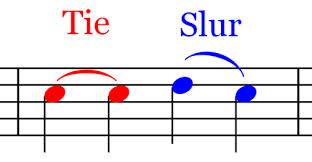
\includegraphics[width=0.5\columnwidth]{./fig/tieslur.jpg}
	\caption{Tie Slurs }
	\label{fig:figure1}
	\end{figure}


\paragraph{Tempo marks}

	\subsection{U}

	\subsection{V}

	\subsection{W}

	\subsection{X}

	\subsection{Y}

	\subsection{Z}








\paragraph{All together}





%	================================================================== Part			분류
%	\addtocontents{toc}{\protect\newpage}
	\chapter{음악 악보}
	\noptcrule
	\parttoc				

	\section{음악 악보}




% ------------------------------------------------------------------------------
% End document
% ------------------------------------------------------------------------------
\end{document}



